\section{Улучшение процедуры SweepB}
Процедура \textsc{SweepB(L, H)} обновляет ранги точек из $H$, сравнивая их с точками из $L$ по первым двум критериям.
Как уже упоминалось в описании алгоритма, оба множества $L$ и $H$ отсортированы лексикографически, что позволяет проходить каждый список ровно один раз слева направо, используя метод заметающей прямой.
Также не будем забывать, что ранги точек из $L$ уже известны и окончательны.

В процедуре поддерживается множество $T$, в котором хранятся <<представители>> встречаемых фронтов точек. Представителем фронта $i$ всегда является точка с рангом $i$ и наибольшим значением по второму критерию. 
Это может быть любое сбалансированное дерево со значением по второму критерию в качестве ключа и номером фронта в качестве значения.

Т.к. мы спускаемся по дереву каждый раз, когда обновляем представителя фронта при итерации по $L$ и каждый раз, когда делаем запрос по второму критерию при итерации по $H$, то общее время работы процедуры --- $O((|L|+|H|)\log{|L|})$.

Пусть $A_i$ --- представитель фронта $i$, $A_j$ --- представитель фронта $j$, и $i < j$.
Тогда по определению: $A_i[0] \leq A_j[0]$ и $A_i[1] \leq A_j[1]$.
Отсюда следует, что при обновлении представителя фронта структура дерева не меняется.
Мы можем воспользоваться этим условием и не спускаться каждый раз по дереву, если фронт текущей точки из $L$ уже встречался.

Введем вспомогательную структуру $P$, массив размера $N$.
В $P[i]$ будем хранить указатель на вершину дерева $T$, где лежит представитель фронта $i$.
Если фронт $i$ еще не встречался, то в $P[i]$ будет лежать нулевой указатель.

\begin{figure}[h]
\centering
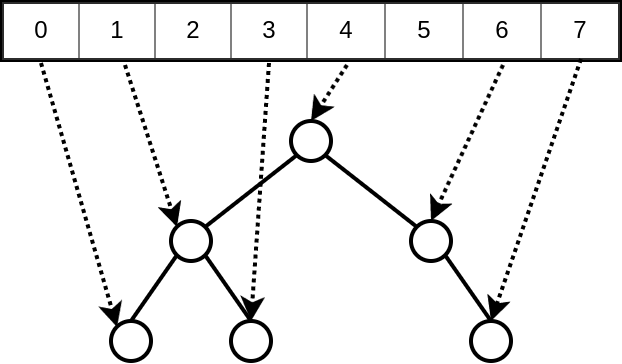
\includegraphics[width=0.7\textwidth]{images/sweep.png}
    \caption{Вспомогательный список указателей в \textsc{SweepB}}
\end{figure}

Таким образом, если ранг текущей точки --- $i$, и в дереве уже лежит какой-то представитель соответствующего фронта, то вместо cпуска по дереву за $O(\log(|L|))$ мы лишь изменим ключ вершины по ссылке $P[i]$ за $O(1)$.

В худшем случае, когда все точки из $L$ имеют различные ранги, время работы остается прежним.
Однако на практике чаще всего встречается ограниченное число рангов, поэтому описанная выше модификация существенно улучшит время работы \textsc{SweepB}.
